%
% File emnlp2020.tex
%
%% Based on the style files for ACL 2020, which were
%% Based on the style files for ACL 2018, NAACL 2018/19, which were
%% Based on the style files for ACL-2015, with some improvements
%%  taken from the NAACL-2016 style
%% Based on the style files for ACL-2014, which were, in turn,
%% based on ACL-2013, ACL-2012, ACL-2011, ACL-2010, ACL-IJCNLP-2009,
%% EACL-2009, IJCNLP-2008...
%% Based on the style files for EACL 2006 by 
%%e.agirre@ehu.es or Sergi.Balari@uab.es
%% and that of ACL 08 by Joakim Nivre and Noah Smith

\documentclass[11pt,a4paper]{article}
\usepackage[hyperref]{emnlp2020}
\usepackage{times}
\usepackage{latexsym}
\usepackage{csquotes}
\usepackage[fleqn]{amsmath}
\usepackage[11pt]{moresize}
\usepackage{anyfontsize}
\usepackage{setspace}
\usepackage{multirow}
\usepackage{subfig}
\usepackage{adjustbox}


\usepackage{xcolor}

\usepackage{mdframed}

\usepackage{makecell}


\usepackage{graphicx}
\usepackage{float}
\usepackage{tabu}
\usepackage{pifont}
\usepackage{latexsym}
\renewcommand{\UrlFont}{\ttfamily\small}

% This is not strictly necessary, and may be commented out,
% but it will improve the layout of the manuscript,
% and will typically save some space.
\usepackage{microtype}

%\aclfinalcopy % Uncomment this line for the final submission
%\def\aclpaperid{***} %  Enter the acl Paper ID here

%\setlength\titlebox{5cm}
% You can expand the titlebox if you need extra space
% to show all the authors. Please do not make the titlebox
% smaller than 5cm (the original size); we will check this
% in the camera-ready version and ask you to change it back.


\newcommand\BibTeX{B\textsc{ib}\TeX}

\definecolor{atomictangerine}{rgb}{0.8, 0.2, 0.1}
\definecolor{turq}{rgb}{0.0, 0.5, 0.5}
\definecolor{darkturq}{rgb}{0.0, 0.4, 0.4}
\definecolor{bright}{rgb}{0.8, 0.1, 0}
\definecolor{darkgray}{gray}{0.3}
\definecolor{gray}{gray}{0.5}
\definecolor{mahogany}{rgb}{0.6, 0.05, 0.05}
% \definecolor{pink}{rgb}{1,0.05,0.6}
\definecolor{myblue}{rgb}{0.3,0.05,0.9}

\definecolor{olive}{rgb}{0.537, 0.627, 0.318}
\definecolor{green}{rgb}{0.22, 0.463, 0.114}
\definecolor{grey}{rgb}{0.4, 0.4, 0.4}
\definecolor{blue}{rgb}{0.435, 0.659, 0.863}
\definecolor{pink}{rgb}{0.761, 0.482, 0.627}
\definecolor{darkpink}{rgb}{0.561, 0.282, 0.427}
\newcommand\darkturq[1]{\textcolor{darkturq}{#1}}
\newcommand\mahogany[1]{\textcolor{mahogany}{#1}}
\newcommand\todo[1]{\textcolor{darkturq}{\textbf{TODO:} #1 }}

\newcommand\darkgray[1]{\textcolor{darkgray}{#1}}

\newcommand\gal[1]{\textcolor{bright}{\textbf{GAL:} #1 }}
\newcommand\yuval[1]{\textcolor{darkpink}{\textbf{YUVAL:} #1 }}
\newcommand\tzuf[1]{\textcolor{blue}{\textbf{TZUF:} #1 }}
\newcommand\reut[1]{\textcolor{green}{\textbf{REUT:} #1 }}

\newcommand\edit[1]{\textcolor{brown}{ #1 }}

\newcommand\ignore[1]{}


\title{ZEST:  Zero-shot Learning from Text Descriptions Enhanced with Textual Similarities and Visual-Descriptions}


\author{First Author \\
  Affiliation / Address line 1 \\
  \texttt{email@domain} \\\And
  Second Author \\
  Affiliation / Address line 1 \\
  \texttt{email@domain} \\}

\date{}

\begin{document}
\maketitle
\begin{abstract}




%when Language and Vision Meet - the vision part the focus is usually on the vision part, while simple models are used for the text representation such as TF-IDF.
%Just a simple attention to the model would do.


%write it is a faster model? how to


We study the problem of classifying images according to unstructured textual descriptions, in a zero-shot setup. That is, in training we get an image of its corresponding class and textual-description of the class. In the zero-shot phase we get a previously unseen image, from a previously unseen set of classes, and we need to assign it to the correct class, where for each class a textual description is assigned.
Previous approaches focus on improving the text representation, by transforming it to focus on the visually similar and different aspects of the different classes. In contrast, we focus on the text representation: (1) we leverage the similarity between images as it is reflected in texts, that is, when the actual classes of the images look similar, the texts are also similar; (2) we extract visual-descriptions from the text, making the text more compatible with the image.
We augment a simple attention-based model with the textual similarity and visual descriptions. 
Our results consistently and significantly outperform the state-of-the-art on the largest benchmarks for Text-based Zero-shot Learning, illustrating the critical importance of the text representation in zero-shot image recognition setups. 

\end{abstract}




\section{Introduction}

\yuval{We need to stress how important this setup is, because the other widespeard attribute-based and caption-based and benchmarks for ZSL are flawed. They rely on raters annotating the attributes (or captions) on images from the \textit{test} set of unseen categories.}

Recent successes of deep learning methods for the task of object recognition are heavily dependent on large dataset collection.
Moreover, the number of categories keeps increasing and with it the need to collect more data. However, this process of collecting millions of images and their corresponding tags is highly expensive and time-consuming. \par




Zero-shot learning aims at overcoming the need to collect data for new categories, by learning the connections between images and auxiliary knowledge about the classes. Thus, the input is an image and auxiliary information about the classes, and the output is the class label. In the zero-shot phase, new classes are given, unseen during training. In the ZSL, the auxiliary information's function is to compensate for the unseen-before visual information.
\par


\begin{figure}[th]
\centering
\scalebox{0.48}{
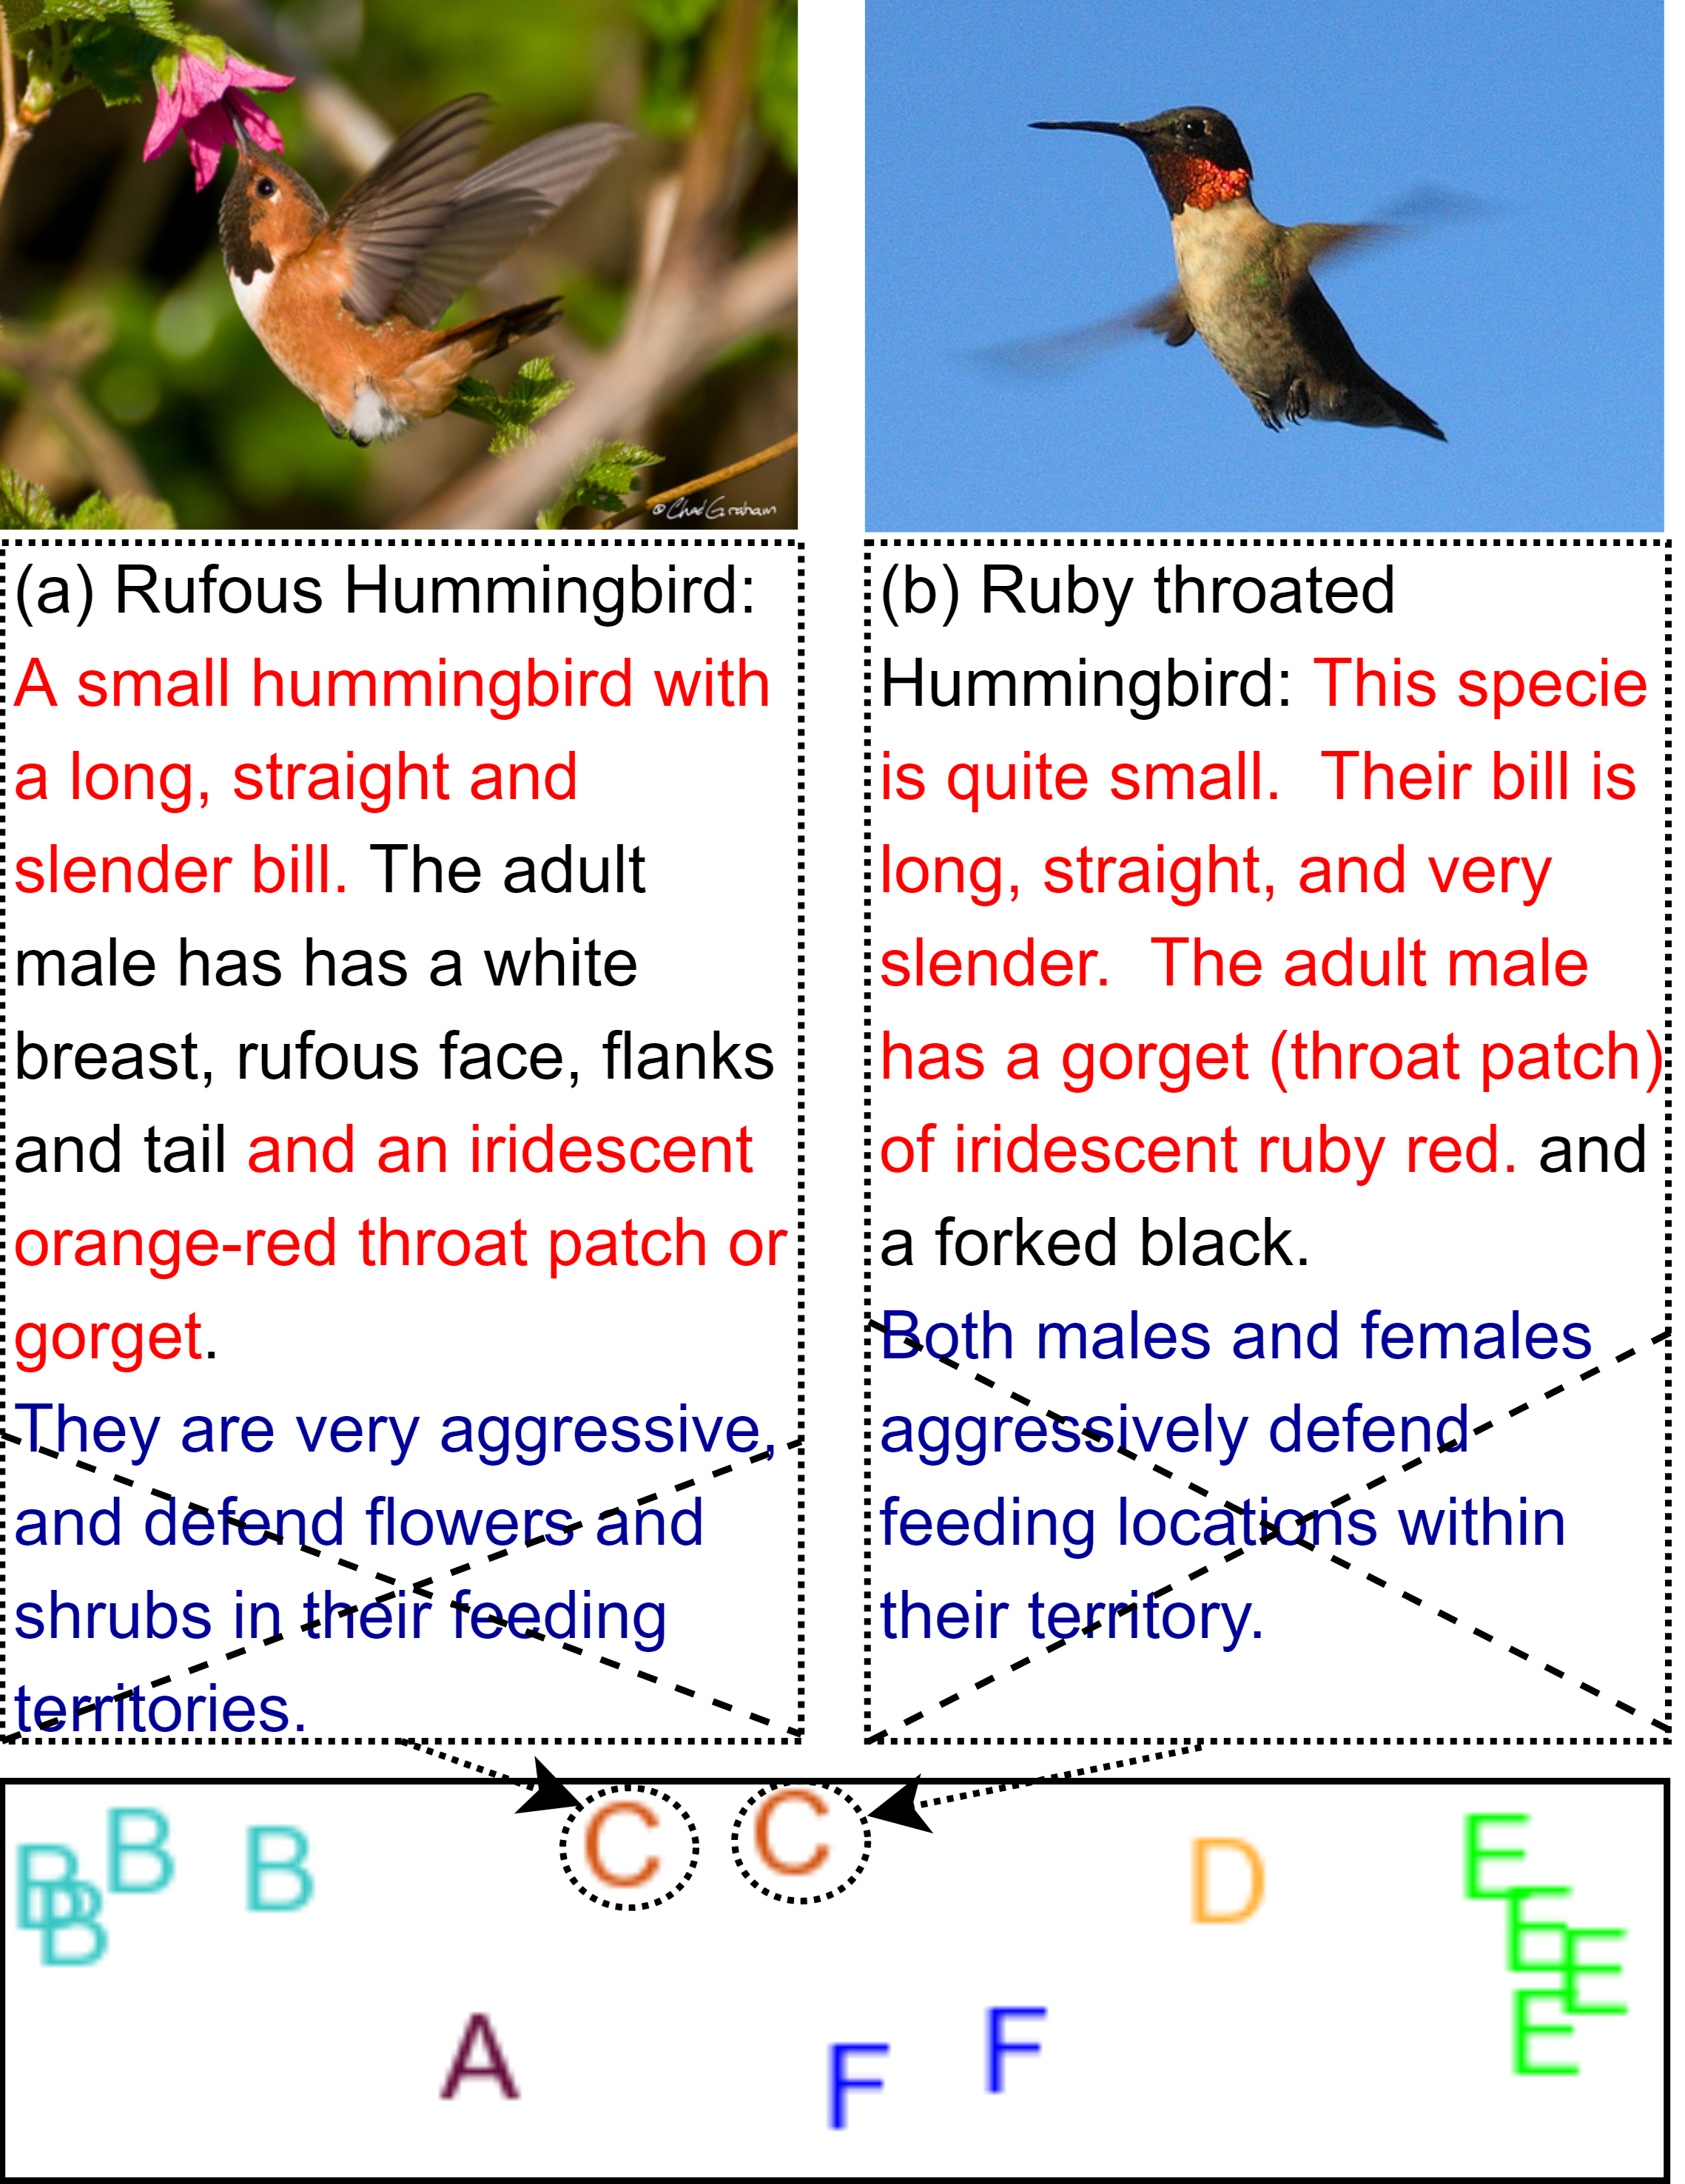
\includegraphics[width=\textwidth]{images/ZEST_text_similarities_visual_descriptions.png}}
 \caption{Textual Similarity and Visual-Descriptions Enhancing: (1) Our approach leverages the similarity and  between texts (red) via clustering (bottom box); (2) non-visual description are removed (blue with X sign). }
 %The red color are components added on top of a standard CGA.}
\label{fig:bird_example}%
\end{figure}

Most previous models for zero-shot image recognition tasks rely on auxiliary information given by experts who manually describe each class by a set of semantically meaningful properties known as attributes (e.g. black-tail for a class of dogs) \citep{farhadi2009describing, lampert2009learning, atzmon2018probabilistic,akata2013label,wang2013unified,changpinyo2016synthesized, akata2015label,ji2018stacked}. \par




Recently a more 
%realistic
applicable
approach was introduced, relying on available online text to describe the classes, thus avoiding the expensive annotation.
Thus, the input of the task is (1) an image; and (2) the text descriptions of the classes as the auxiliary information. \par

To get an intuition of the task consider the following situation:
imagine you never saw a zebra in your life but know how a horse looks like. What if you were given a text describing a zebra: \enquote{Zebras have hooves, mane, tail, pointed ears, and white and black stripes}. This description would probably be very close to a description of a horse and you would probably be looking for an image that reminds you of a horse but has \enquote{white and black stripes}. Thus, without previously knowing what a zebra is, using text-descriptions of the zebra, one can correctly classify unknown categories like a zebra.

Our task raises many challenges: (1) our images in this task are of birds, and as the differences between the birds are small, it is a fine-grained classification task; (2) This is an expert task, which is hard for non-bird-experts to complete, as in addition to the small difference between the birds, the text contains terminology for describing a bird that is not likely to be familiar to a layman;
(3) The text descriptions of the classes are long and very noisy. \par 


The ZSL task contains two real scenarios: (1) an \enquote{easy} scenario where we see a new unknown object that is similar to a previously known object; (2) a \enquote{hard} scenario where the new object is different from known objects, thus, the relevance between seen and unseen objects is minimal.\par

Continuing with our previous example of zebras and horses, we note that that similar objects (images) have similar texts and that in order to differentiate between the objects we need to consider the visual-descriptions of the text.  Thus, in an easy scenario where the horse is known to us but the zebra is not - we can benefit from the similarity between the objects and texts. Whereas in a hard scenario we know neither the class of horses or zebras, and we want to classify a new images as horse or zebra. This requires that we enhance the visual differences in the text.\par

In this work, we focus on the text representation, and ask the question: which aspects of the text are important for classifying images? We use the intuitions given in the horse-zebra example: (1) that similar objects (images) have similar texts - to create a kernel-like method to enhance separability of texts that reflects real similarity of the objects; (2) that the differences are salient visual features in the text - by extracting visual descriptions of the text, thus, enhancing the compatibility of the text and the image (see Figure \ref{fig:bird_example}).\par

\par


Our experiments empirically demonstrate the 
efficacy of either of our methods. 
In experiments carried out on two fine-grained datasets with two different splits, the similarity method obtains a ratio improvement of up to 18.3\% and with the addition of extracting visual description we obtain a ratio improvement of up to 48.16\% over the state-of-the-art.

Furthermore, we show the generality of our VS method by showing generalizability across datasets, and by showing its contribution to additional SOTA Models by a ratio improvement of up to 59.62\%.



Our main contributions are as follows:  
\begin{enumerate}
  \item We show the importance of text in zero-shot image recognition by showing two distinct text-based processing methods that vastly improve the results.
  
\item We demonstrate the efficacy and generalizability of the method by applying the proposed methods to the zero-shot learning task and the generalized-zero shot task, out preforming all previously reported results.
    

\end{enumerate}

The significance of the improvement of our text processing methods, on a variety of models, implies value in applying text processing methods in future research, in tasks which include vision and language modalities.


\par


\section{Related Work}


Text-based zero-shot learning is a multimodal learning task, composed of three parts: (1) text representation (2) image-representation (3) a compatibility function between the two modalities: image and text. \par

Previous works focused mainly on the latter two parts: improving the image representation and the compatibility function. In this work, we focus on the text modality. \par

In the image modality many studies that do ZSL for object recognition \cite{xu2018attngan,lei2015predicting,qiao2016less,akata2016multi}, rely on features extracted using the well-established method of
Convolutional Neural Network (CNN) \cite{lecun1995convolutional}. More recent works, use object detection methods to detect parts of the object and extract visual features at the part-level \cite{elhoseiny2017link,zhu2018generative,zhang2016spda}. This
method makes the image more compatible with the text, as it enables text-terms such as \enquote{crest} to be linked to the visual representation of parts like \enquote{head}. \par



There are different approaches as to the function that learns compatibility function between images and their textual descriptions: (1) \textbf{Visual-to-Semantics:} learning a function that maps from the visual space to the semantic space \citep{socher2013zero}. Thus, if one has an image, the function predicts the correct text related $F(X)=Y$ where X is the images and Y the texts; (2) \textbf{Semantics-to-Visual:} learning a function from the semantic space to the visual space \citet{zhu2018generative} $F(Y)=X$. This can be done by generating images from text, thus, the problem becomes a \enquote*{regular} classification problem as we now have generated images with the corresponding text labels; (3) \textbf{Joint learning:} simultaneously learns a function from the semantic and visual space to a common space and predicts a compatibility score: $F(X,Y)=score$  \cite{akata2015evaluation,akata2016multi,qiao2016less,elhoseiny2013write,elhoseiny2016write}.\par



\begin{figure*}[t]
\centering
\scalebox{1}{
\includegraphics[width=\textwidth]{images/ZEST_model_4.png}}
 \caption{Our ZEST$_{similarity}$+VS model with similarity component and Visually-Focused Summarization (VS) component.}
\label{fig:data}
\end{figure*}

In this work, we adopt the third approach and aim to process the textual modality in order to increase the compatibility between textual features and visual features, that can be detected by the learning architecture.
\par

Most studies to date have used an impoverished text representation such as Bag-of-Words (BOW) and Term Frequency-Inverse Document Frequency (TF-IDF) and focused on improving the visual representation and the model \cite{lei2015predicting,elhoseiny2013write,elhoseiny2016write,elhoseiny2017link,zhu2018generative}. Beyond that, \citet{qiao2016less} used a simple BOW and a l2,1-norm based objective function to suppress the noisy signal in the text. However, this impoverished treatment of the text side is problematic, as the text contains key information to the correct class. 

In this work we aim to establish the importance of adequately processing the text side, to obtain a sound representation of the features most salient for the task. This is done to complement the work done on the visual modality, that aimed to increase image compatibility with the text.





\section{Proposed Approach}
\label{task}

The key idea we would like to propose is to transform the text representation from a non-task-oriented representation to a task-oriented representation of the most salient features for the visual recognition task. More specifically, instead of letting the text representation encode a broad class description, we designed a representation that encodes salient features that are relevant for the classification. We do this by employing two different (complementary) methods: (1) text similarities; and (2) extraction of visual-description from the text.


\subsection{Basic Architecture (ZEST$_{vanilla}$)}
\label{section_ZEST_C}


Our basic, vanilla, architecture is a simple multiplicative attention mechanism \cite{luong2015effective} inspired by \citet{romera2015embarrassingly}. We model the problem using an attention-based model, where the image $x$ is queried
%considered 
against the candidate documents of the classes D.


\begin{equation}
\label{equation:attention}
\begin{aligned}
\begin{split}
&f(x,D)=x^TWD
\end{split}

\end{aligned}
\end{equation}

 We then take the candidate $d$ with the maximum score, and obtain the most probable label  $y$ for this image:

\begin{equation}
\label{equation:attention}
\begin{aligned}
\begin{split}
&y={argmax}_{d\in D}f(x,D)
\end{split}

\end{aligned}
\end{equation}

Where $d\in D$ is the document in the set of documents $D$ that receives the maximum score on the dot product with $x$. 



\begin{figure}[t]
\centering
\scalebox{0.42}{
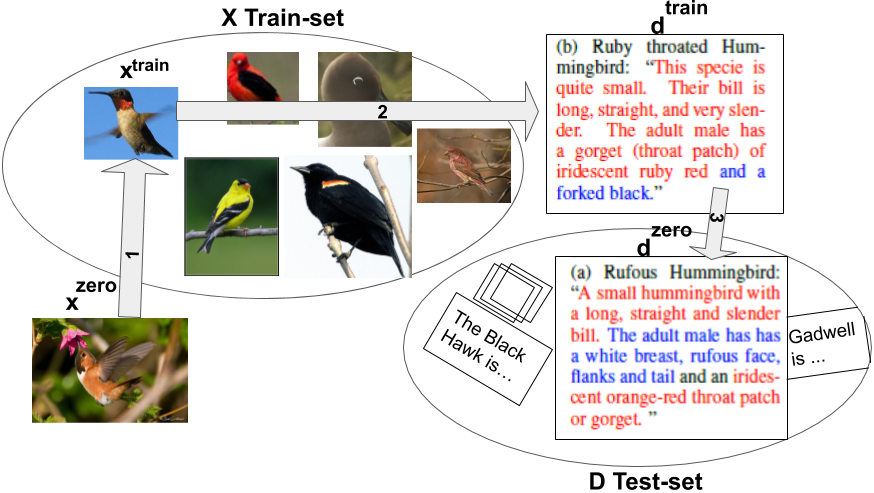
\includegraphics[width=\textwidth]{images/DS_model.png}}
 \caption{Deterministic Similarity (DS) Model}
\label{fig:DS}
\end{figure}

\subsubsection{Image Encoder}
\label{section:Image_Encoder}
The goal of the visual encoder is to transform the image to a vector representation of the most salient visual features for the classification.\par

We adopt a 
Fast Region-based Convolutional Network framework (Fast R-CNN) for object detection   \citep{girshick2015fast} to detect seven semantic parts in the CUB dataset:
\enquote{head},\enquote{back},\enquote{belly},\enquote{breast},\enquote{leg},\enquote{wing},\enquote{tail}.\par
This image-representation method was present by \citet{zhang2016spda} and applied to the text-based ZSL task \cite{zhu2018generative,elhoseiny2017link} . \par

The images are first encoded by VGG16 architecture \citep{simonyan2014very} and then visual features are extracted from parts detected using Region of Interest Pooling pooling (ROI) layer \citep{girshick2015fast}. %add cite to ROI pooling
The encoded features of each visual part are then concatenated into a feature vector which functions as the image representation for the text-based ZSL.


\subsubsection{Basic Text Encoder}
\label{section:Text_Encoder}
Our basic encoder processes the text into a feature vector. It is a Term Frequency-Inverse Document Frequency (TF-IDF)  representation \citep{salton1988term}, which requires the following pre-processing: (1) tokenization of the words; (2) stop words are removed; (3) stemming is performed on the remaining words; (4) Finally, we extract a feature vector using TF-IDF. This processing procedure is similar to the text processing presented by \citet{zhu2018generative}.
The dimensionalities of TF-IDF features for
CUB and NAB are 7551 and 13217 respectively. 


\subsection{The Importance of being Similar}

We leverage the similarities between images and texts. Meaning, when the actual classes of the images look similar, the texts are also similar.

Similarities between texts reflect on real similarities between objects. We want to reconstruct this analogy-link.


The TF-IDF representation of a text is on the word-level: representing the uniqueness of a word in the document and between documents. However, this word-level representation of similarity does not take document level similarities into account. \par

\par

Our intuition is that similarities between texts will suggest a similarity between objects, and vice versa. To test this intuition we propose two models: (1) a deterministic model (2) adding a similarity component to our stochastic model ZEST$_{vanilla}$.

For both models we use the Image Encoder (section \ref{section:Image_Encoder} to process the images $x$, and the Text Encoder (section \ref{section:Text_Encoder}) to process documents D.

\subsubsection{Deterministic Similarity (DS) Model}

Our approach leverages the analogy between images and texts. Figure \ref{fig:DS} presents our Deterministic Similarity (DS) Model. Given an image $x^{zero}$ in the zero-shot phase we: (i) look for the cosine similarity between $x^{zero}$ and all the images from training $X^{train}$. We get image $x^{train}$; (ii) image $x^{train}$ corresponds to document $d^{train}$ (iii)
look for the cosine similarity between $d^{train}$ and all the texts from zero-shot phase $D^{zero}$. We achieve the document $d^{zero}$ which corresponds to the label $y$:


The following equation follows step (i) and (ii):

\begin{equation}
\begin{aligned}
\begin{split}
&d^{train}= \\
&D^{train}[
\operatorname*{argmax}_{x^{train}\in X^{train} } \frac{<x^{zero},X^{train}>}{\norm{\| x^{zero}\| }*\norm{\| X^{train}\| }}]
\end{split}

\end{aligned}
\end{equation}

The following equation follows step (iii):

\begin{equation}
\begin{aligned}
\begin{split}
&y=Y^{zero}[
\operatorname*{argmax}_{d\in D^{zero}} \frac{<d^{train},D^{zero}>}{\norm{\| d^{train}\| }*\norm{\| D^{zero}\| }}]
\end{split}

\end{aligned}
\end{equation}

\subsubsection{ZEST$_{similarity}$}

Having established the importance of similarity, here we embed it into our stochastic ZEST$_{vanilla}$, to benefit from it in the learning procedure. \par

We take a kernel-like approach, aiming to transform the text space into a linearly separable space, where sets of texts are separable. \par

The Basic Encoder used allows us to see similarities and differences on the word-level. However, we want to find similarities on the document level. To achieve that, we add our $similarity$ component which clusters training and test texts. If over 15\% of the texts from test-set are clustered with at least one text from train-set we concatenate the encoded cluster label to the document representation $d$. \par

This similarity-difference representation is then passed as an input to the ZEST$_{vanilla}$ model (\ref{section_ZEST_C}). \par

We hypothesize that the similarity component will work well on the \enquote{easy} scenario - where closely related birds are seen during training. \par

\subsection{The Importance of Being Seen (ZEST$_{similarity}$+VS)}

While the similarity method takes advantage of the similarity between objects seen in training and test, here we want to address the scenario where similar objects are seen during test time only (e.g. zebras and mules). To differentiate between closely related classes in the test-set we need to emphasize the parts that are both different in the image and the text - the visual features. \par

Our aim here is to extract salient visual features in the text, thus, making the text more compatible with the image. 

 \par
 
\subsubsection{Visually-Focused Summarization (VS)}


Our method for enhancing visual description is based on a Visually-Focused Extractive Summarization (VS).

Extractive summarization is the task of extracting a small number of sentences that summarizes a given document.
In this work we define: Visually-Focused Extractive Summarization (VS) as the task of extracting only sentences that contain visual-descriptions. A \enquote{naive} approach would be to extract sentences that we know are visually salient in our domain (e.g., the 7 parts employed by the vision recognition representation).  However, this naive approach has the following drawbacks: (1) bird parts can be described in many different terms; (2) a bird can be described by its color, without any mention of a body-part. 
Instead, we propose to use similarity between sentences containing visual-descriptions. According to this approach, if we want to extract sentences that contain visual-descriptions than we need to compare the similarity between sentences in the document and other sentences that happen to visually describe these kinds of objects. 
\par
Note that we cannot rely on descriptions of particular species (due to the zero-shot setup), and have to do with descriptions of objects in the family that can be naturally obtained for the general class of objects we are interested in.\par

Such naturally occurring descriptions are, for instance, captions of bird images. (not necessarily those species from our dataset). We use a set of captions to create an unsupervised classifier that predicts whether a sentence is relevant, that is, whether it contains descriptions that can be seen in an image.
%We use only captions of birds that are seen during training.
For each document we do pairwise similarity between captions and sentences and assign a score to each sentence.

We embed both captions ($c_{0:N}$) and sentences ($s_0:M$) in the document with BERT \cite{devlin2018bert} and a pre-trained siamese network framework developed by \citet{reimers2019sentence}. The score of sentence $s$ is defined as:

\begin{equation}
\begin{aligned}
\begin{split}
\label{eq:score}
&score(s)=  \frac{1}{N}
&\sum_{i=0}^{N} \frac{c^i\cdot s}{ \norm{\| s\| }}
\end{split}
\end{aligned}
\end{equation}

 We then extract only the top 30 sentences or $\frac{3}{4}$ of the sentences in the document, whichever is lower.\par   

\par




Our documents contain many non-visual descriptions that are unobserved in the images. However, these non-visual descriptions might still be important to the similarity comparison of the documents (e.g. similar-looking birds are likely to be in the same habitat). Thus, the visual-descriptions extraction and the similarity enhancing are done parallel on the original document. We then concatenate the similarity embedding and the visual-descriptions embedding of the text and perform the multiplicative attention on the encoded documents and image.

\section{Experiments}

\subsection{Experiment setting}

\paragraph{Datasets:}  We evaluate our method on the Caltech UCSD Birds-2011 dataset (CUB) \citet{wah2011caltech} and the North America’s birds dataset (NAB) \cite{van2015building}, using text class description obtained from wikipedia and AllaboutBirds website \footnote{https://dl.allaboutbirds.org/bayareafocusgroup} collected by \citet{elhoseiny2017link}. 
Both are datasets of birds, with small differences in the images and texts, making it a challenging task of fine-grained classification. The CUB dataset contains 11,788 images of 200 bird species, and the NAB
is a larger dataset of birds with 48,562 images of 404 classes \footnote{\citet{elhoseiny2017link} merged the original 1,011 classes according to the subtle division of classes.}.
In addition, the texts of both CUB and NAB are long, containing much irrelevant information. CUB has an average of 869 tokens and 42 sentences per document of a class. NAB has an average of 1277 tokens and 58 sentences per document of a class. 

\paragraph{Two split Settings} We use the two splits for both datasets presented by \citet{elhoseiny2017link}: (1) Super Category-Shared (SCS) also referred to as the \enquote*{easy} split; and (2) Super-Category-Exclusive (SCE) also referred to as the \enquote*{hard} split. The SCS-split for each class in the test-set, at one class in the training belongs to the same category (categories are organized taxonomically). E.g. in Figure \ref{fig:bird_example}, the Rufous Hummingbird and the Ruby-throated Hummingbird are both from the Hummingbird category. In the SCE-split scenario, all the classes in a category are in the same set, such that, if a class is in the test-set then other classes from the same category will be in the test-set. Intuitively, classes from the same category have high similarity in both images and texts, so that in the SCE-split scenario a class is seen for the first time but a very similar looking bird was seen in training, making it easier than the SCS.

\paragraph{Clustering Algorithms:}
The parameters of our model include clusters parameters.
We use two clusters methods: (1) Density-based spatial clustering of applications with noise (DBSCAN) \citep{ester1996density}; (2) Hierarchical DBSCAN \citep{mcinnes2017hdbscan}.
We optimize the parameters on a validation set. The ZEST$_{vanilla}$, ZEST$_{similarity}$, and ZEST$_{similarity}$+VS are trained using categorical cross-entropy.
%optimization loss

\paragraph{Human Summarization:} 
In order to test our visual-description extraction approach, we wanted to conduct an oracle experiment where the ground-truth is a visually-focused summarization is tested. To this end we manually created a ground-truth visually-focused summarization by going over all the sentences in the CUB dataset, and tagging them as including or excluding visual descriptions of the bird in question. Only 11.9\% of the sentences were found to include visual descriptions.  

\paragraph{Image Captions:}
To create Visual summaries we use the captions provided by \citet{reed2016learning} for the training images of birds. To showcase the generality of this approach we use these captions in both in-domain (CUB) and out-of-domain (NAB) scenarios.
Each image in the CUB dataset has been annotated with 5 fine-grained captions. These captions describe only the visual appearance of the birds while avoiding mentioning the name of the bird species. E.g. \enquote{This bird has a long beak, a creamy breast, and body, with brown wings.} Image captions 
are used only in the ZEST$_{similarity}$+VS model.
\par

We limit the use of caption to those that correspond to  images that are seen during training in the CUB dataset. In the NABirds all caption from the CUB dataset are allowed.


\paragraph{Baselines:}  The performance of
our approach is compared to ten leading algorithms (see Table \ref{tab:results}): MCZSL\citep{akata2016multi}, WAC-Linear \citep{elhoseiny2013write}, Wac-Kernel \citep{elhoseiny2016write}, ESZSL \citep{romera2015embarrassingly}, SJE \citep{akata2015evaluation}, Sync$_{fast}$ \citep{changpinyo2016synthesized}, Sync$_{OVO}$ \citep{changpinyo2016synthesized},
ZSLNS \citep{qiao2016less}, and GAZSL \citep{zhu2018generative}. 




\paragraph{Generalized Zero-Shot Learning:} 
The conventional zero-shot learning task considers the candidate class from unseen classes only. However, in a realistic scenario seen objects might also appear \cite{chao2016empirical}. In Generalized Zero-Shot Learning (GZSL), test data might also come from seen classes and the labeling space is the union of both types of classes. We follow \citet{chao2016empirical} metric, and used also by \citet{zhu2018generative}, to evaluate our models on the GZSL task. We evaluate the accuracy of the Seen-Unseen accuracy Curve (SUC) and use Area Under SUC to measure the general capability of methods for ZSL.



 \begin{table}[t]
  \centering
 \scalebox{0.6}{

\begin{tabular}{l|ll|ll} 
\Xhline{6\arrayrulewidth}
\multirow{2}{*}{\textbf{ methods} }                                  & \multicolumn{2}{c|}{\textbf{CUB } }                                    & \multicolumn{2}{c}{\textbf{NAB} }                                     \\ 
\cline{2-5}
                                                                     & \multicolumn{1}{c}{\textbf{SCS} } & \multicolumn{1}{c|}{\textbf{SCE} } & \multicolumn{1}{c}{\textbf{SCS} } & \multicolumn{1}{c}{\textbf{SCE} }  \\ 
\hline
Random pick                                                          & 2                                 & 2.5                                & 1.23                              & 1.23                               \\ 
\hline
MCZSL \citet{akata2016multi}                        & 34.7                              & -                                  & -                                 & -                                  \\
WAC-Linear \citet{elhoseiny2013write}          & 27.0                              & 5.0                                & -                                 & -                                  \\
WAC-Kernel \citet{elhoseiny2016write}              & 33.5                              & 7.7                                & 11.4                              & 6.0                                \\
ESZSL \citet{romera2015embarrassingly}              & 28.5                              & 7.4                                & 24.3                              & 6.3                                \\
SJE \citet{akata2015evaluation}                    & 29.9                              & -                                  & -                                 & -                                  \\
ZSLNS \citet{qiao2016less}                          & 29.1                              & 7.3                                & 24.5                              & 6.8                                \\
SynC$_{fast}$ \citet{changpinyo2016synthesized}     & 28.0                              & 8.6                                & 18.4                              & 3.8                                \\
SynC$_{OVO}$ \citet{changpinyo2016synthesized}      & 12.5                              & 5.9                                & -                                 & -                                  \\
ZSLPP \citet{elhoseiny2017link}                   & 37.2                              & 9.7                                & 30.3                              & 8.1                                \\
GAZSL \citet{zhu2018generative}                   & 43.7                              & 10.3                               & 35.6                              & 8.6                                \\ 
\hline
Deterministic Similarity (DS) & 40.402                            & 5.551                              & 37.002                            & 5.517                              \\
ZEST$_{vanilla}$                                                                 & 39.16                            & 11.77                             & 27.61                            & 10.18                             \\
\textbf{ZEST$_{similarity}$}                                           & \textbf{47.48}                   & \textbf{11.77}                     & \textbf{38.2}                   & \textbf{10.18}                    \\
\hline
\textbf{ZEST$_{similarity}$+VS}                                        & \textbf{48.57}                    & \textbf{15.26}                    & \textbf{38.51 }                   & \textbf{10.23 }                    \\ 
\Xhline{6\arrayrulewidth}
                 
\end{tabular}
}
\caption{Top-1 accuracy (\%) on CUB and NAB datasets with two split settings.}
\label{tab:results}
\end{table}


\begin{table}[t]
\centering
 \scalebox{0.61}{
\begin{tabular}{l|cc|cc} 
\Xhline{6\arrayrulewidth}
\multirow{2}{*}{\textbf{ methods} } & \multicolumn{2}{c|}{\textbf{CUB } }                                                              & \multicolumn{2}{c}{\textbf{NAB} }           \\ 
\cline{2-5}
                                    & \textbf{SCS}                                    & \textbf{SCE}                                   & \textbf{SCS}         & \textbf{SCE}          \\ 
\hline
GAZSL                               & \begin{tabular}[c]{@{}c@{}}43.74\\\end{tabular} & \begin{tabular}[c]{@{}c@{}}10.3\\\end{tabular} & 35.6                 & 8.6                   \\
GAZSL+parts summarization                               & \begin{tabular}[c]{@{}c@{}}19.54\\\end{tabular} & \begin{tabular}[c]{@{}c@{}}9.557\\\end{tabular} & 23.32
                 & 7.2
                   \\
GAZSL+parts summarization +${similarity}$                               & \begin{tabular}[c]{@{}c@{}}38.25\\\end{tabular} & \begin{tabular}[c]{@{}c@{}}9.557\\\end{tabular} & 33.05
                 & 7.2
                   \\
GAZSL+VS                            & 43.72                                           & \textbf{16.44}                                       & 37.28
                & 9.237                 \\
GAZSL+HUMAN                         & 35.98                                           & 21.81                                          & -                    & -                     \\
GAZSL+HUMAN+${similarity}$                       & 47.32                                           & 21.81                                          & -                    & -                     \\ 
\hline
ZEST$_{similarity}$                                & 47.48                                           & 11.77                                          & 38.2
                & 10.18                 \\
ZEST$_{similarity}$+parts summarization                                & 42.27
                                           & 10.93
                                          & 37.02

                & 8.055
                 \\
            ZEST$_{vanilla}$                                                                 & 39.16                            & 11.77                             & 27.61                            & 10.18                             \\
                
                 
  ZEST$_{vanilla}$+VS                             & {42.58}                                  & {15.26}                                 & {32.24}      & {10.23}        \\
ZEST$_{similarity}$+VS                             & \textbf{48.57}                                  & {15.26}                                 & \textbf{38.51}      & \textbf{10.23}        \\

ZEST$_{similarity}$+HUMAN                          & 48.99                                & 17.2                                           & -                    & -                     \\ 
\Xhline{6\arrayrulewidth}
\end{tabular}
}
    \caption{Visually-Focused Summarization (VS) added to GAZSL, and to ZEST$_{similarity}$. Improvement across on all splits and models, due to applying VS. }%
    \label{table:summarization}%
\end{table}





\begin{table}[t]
\centering
 \scalebox{0.87}{
\begin{tabular}{l|c|c} 
\Xhline{6\arrayrulewidth}
                                & \textbf{CUB }  & \textbf{NAB }   \\ 
\hline
\textbf{methods }               & \textbf{SCS }  & \textbf{SCS }   \\ 
\hline
ZEST$_{vanilla}$                     & 39.16          & 27.61          \\
ZEST$_{vanilla}$ + bird category  & 43.71          & 36.73           \\
Zest$_{vanilla}$ + 1 cluster             & 46.55          & 35.94           \\
Zest$_{similarity}$ (with 2 cluster) & \textbf{47.48} & \textbf{38.2}   \\
\Xhline{6\arrayrulewidth}
\end{tabular}
}
    \caption{Zest model with different Similarity methods }%
    \label{table:similarity}%
\end{table}




\begin{table}[t]
\centering
 \scalebox{0.76}{
\begin{tabular}{l|cc|cc} 
\Xhline{6\arrayrulewidth}
                  & \multicolumn{2}{c|}{\textbf{CUB } } & \multicolumn{2}{c}{\textbf{NAB } }  \\ 
\hline
\textbf{methods } & \textbf{SCS }   & \textbf{SCE }     & \textbf{SCS }   & \textbf{SCE }     \\ 
\hline
ESZSL             & 0.185           & 0.045             & 0.092           & 0.029             \\
ZSLNS             & 0.147           & 0.044             & 0.093           & 0.023             \\
WAC$_{kernal}$         & 0.225           & 0.054             & 0.007           & 0.023             \\
WAC$_{linear}$         & 0.239           & 0.049             & 0.235           & -                 \\
SynC$_{fast}$          & 0.131           & 0.040             & 0.027           & 0.008             \\
SynC$_{OvO}$           & 0.017           & 0.010             & 0.001           & -                 \\
ZSLPP             & 0.304           & 0.061             & 0.126           & 0.035             \\
GAZSL             & 0.354           & 0.087             & 0.204           & 0.058             \\ 
\hline
ZEST$_{similarity}$              & \textbf{0.443 } & \textbf{0.1 }     & \textbf{0.267 } & \textbf{0.067 }   \\
\hline
ZEST$_{similarity}$+VS           & 0.437           & 0.147             & 0.26            & 0.084             \\
ZEST$_{similarity}$+HUMAN        & 0.445           & 0.163             & -               & -                 \\
\Xhline{6\arrayrulewidth}
\end{tabular}
}
    \caption{Generalized Zero-Shot Learning: AUC of Seen-Unseen Curve.  }%
    \label{table:GZSL}%
\end{table}




\subsection{Results}

Table \ref{tab:results} shows the top-1 accuracy
on (1) the top box is the random pick of classes; (2) the second box is previous works; (3) the third box is our proposed models which are comparable to the previous works seen; (4) Our model that uses an additional data - captions. \par 

\paragraph{DS Model:} 
According to table \ref{tab:results} we can see that, for the DS easy-split, the DS model achieves competitive results on the SCS-split to previous methods - 40.402\% on CUB and 37.002\% on NAB. The high scores on the SCS-split, where similar birds are seen in training, is expected, as this method relies on similarities between texts and similarities between images.
In contrast, the DS suffers from low accuracy on the hard-split, as this split doesn't contain birds from the same category in training as the birds in the zero-shot phase. As the DS model relies on the similarity between birds in the zero-shot phase and training, the low accuracy suggests that birds from different categories are less likely to look alike, which is intuitive. 

\paragraph{ZEST$_{vanilla}$}
In contrast to the very sophisticated approaches of \citet{zhu2018generative}, our simple stochastic text-based approach outperforms all previous methods on the SCE-split on both CUB (+14.27\% ratio of improvement) and NAB (+18.37\%  ratio of improvement). As the SCE-split is a more challenging split, this sheds light on the strength of this simple framework.  

\paragraph{ZEST$_{similarity}$}
Next we embed the similarity approach seen in the DS model into the stochastic system as we want to combine the strength of the ZEST$_{vanilla}$ on the SCE-split with the similarity strength presented in the DS model on the SCS-split.
The ZEST$_{similarity}$ model adds the similarity to the representation of the text-only when similar texts are found. Thus, in the case of the SCE-split no similarities are found, and the ZEST$_{similarity}$ preforms as the ZEST$_{vanilla}$ model. 
The combination of a simple yet strong framework as the ZEST$_{vanilla}$ that achieves state-of-art of the SCE-split and the similarity addition- achieves state-of-the-art on all split, in both CUB and NAB datasets. \par


The two clustering algorithms we applied find real similarities, achieving high accuracy in predicting the correct label according to the taxonomic category - 88\% and 84.5\% accuracy on the CUB, and 93.07\% and 95.05\% on the NAB. 

In Table \ref{table:similarity} we can see a comparison between different similarity enhancing methods. The use of two clusters that capture different similarities improves our model over an embedding of the bird category in the text representation, by an absolute improvement of up to 3.77\%.
\par

In Table \ref{table:GZSL} we present the results of ZEST$_{similarity}$ on the GZSL setup. On both datasets and splits, the ZEST$_{similarity}$ achieves the state-of-the-art with up to 30.88\% ratio improvement.

\paragraph{ZEST$_{vanilla}$+VS and ZEST$_{similarity}$+VS }
The ZEST$_{vanilla}$+VS and  ZEST$_{similarity}$+VS models use the captions from training images in the CUB. 

We test the summarized representation on the ZEST$_{vanilla}$ model, the ZEST$_{similarity}$ and the GAZSL \citep{zhu2018generative} model. In Table \ref{table:summarization} we show the experimental results. We compare the models before and after the use of the Visually-Focused  Extractive Summarization component. We see an improvement in accuracy in both models on both datasets and on both splits. The GAZSL improves especially on the SCE-split, as the similarity between texts is reduced. In contrast the ZEST$_{similarity}$ with the similarity component handles the SCS-split, having a component that enhances the similarity in the text representation.  \par

In addition, we see a drop in the \citep{zhu2018generative} performance on the SCS-split. This is because the summarization process of the text reduces the similarity which is important in the SCS-split. However, when adding our similarity model to the \citep{zhu2018generative} with human text summarized (GAZSL+HUMAN+$similarity$) the performance goes up again.
\par  

To asses the quality of the VS summarization performance we treat HUMAN summarization as the ground truth. The VS method succeeds in removing 49.4\% of the sentences in on the CUB dataset with 96.23\% recall and 22.59\% precision. For comparison, removing 49.4\% of the sentences randomly produces a recall of 50.06\% and a precision of 11.9\%.
Another comparison we made is to a state-of-the-art extraction summarization model such as  Textrank \citep{mihalcea2004textrank} algorithm, which achieves a recall of 12.33\% and a precision of 12.83\%.

\par
We then compare both ZEST$_{similarity}$ and the GAZSL to the use of HUMAN summarization in the CUB dataset and see additional improvement in both models on the two splits. The gap between the performance on the Visually-focused summarization and the Human summarization indicates that improvement in the summarization of documents will improve the models' performance, and is, therefore, a promising path for text-based zero-shot learning research.\par


\begin{figure}[t]
\centering
\scalebox{0.42}{
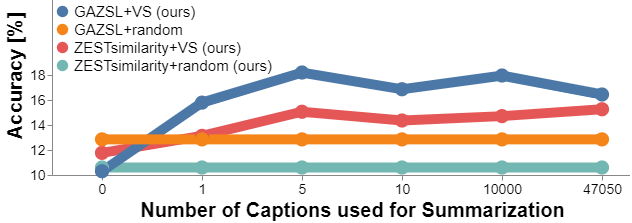
\includegraphics[width=\textwidth]{images/captopm_graph_3.png}}
 \caption{Accuracy per the number of captions used for summarization, measured on the hard Super-Category-Exclusive split (SCE) of CUB. It demonstrates that even 5 captions are sufficient to guide the visually-focused summarization module.}
\label{fig:captions}
\end{figure}


Finally we experiment to assess the number of captions needed for the VS method. The results are seen in Table \ref{fig:captions}. The results show that only a few (~5) captions are needed to achieve the maximum accuracy with this method.  Thus, the VS method does not require using crowdsourcing to produce image captions. 



\par



\section{Conclusion}
\label{conclusion}

This work aimed to establish a better way to represent the text, one which will support text-based ZSL task. Our text-processing methods' significant achievements, prove that text-processing methods are an essential process in text-based ZSL tasks, or indeed, in any vision and language-based tasks. We thus, recommend applying text-processing methods in future research which includes vision and language modalities.


\bibliography{emnlp2020}
\bibliographystyle{acl_natbib}
\end{document}
